\exercise

Let us given the set of strings $S = \{ \text{\tt aabb}, \text{\tt aaabbb},
\text{\tt abbbc}, \text{\tt abbbd}, \text{\tt abbbe}, \text{\tt abc} \}$
%
\begin{enumerate}
    \item Show the Front-Coding compression of $S$;

    \item Show the Locality-Preserving Front-Coding compression of $S$, setting
    $c = 1$ (for simplicity) and counting previous characters and digits for
    ``backward copy-check'' in the LPFC-algorithm;

    \item Describe a two-level index that uses in internal memory a Patricia
    trie on 2 strings;

    \item Show how it is searched the string {\tt aaabba} in that 2-level index.

\end{enumerate}

\solution

\begin{enumerate}

  \item To achieve a better compression, we first sort the strings in $S$ and
  then apply front-coding, obtaining $FC(S) = \{ (0, \text{\tt aaabbb}), (2,
  \text{\tt bb}), (1, \text{\tt bbbc}), (4, \text{\tt d}), (4, \text{\tt e}),
  (2, \text{\tt c}) \}$\footnote{This might be a typo in the text: only the
  first two strings do not respect the lexicographic ordering, so the result
  does not change much. In the third and fourth point, instead, sorting is
  fundamental since we need it for a lexicographic search.}.

  \item Given the first pair $(0, \text{\tt aabb})$, we have that
  %
  \begin{itemize}

    \item $|\text{\tt aaabbb}| > c \cdot |\text{\tt aabb}| \Longrightarrow$
    \emph{copy};

    \item $|\text{\tt aabb}| \le c \cdot |\text{\tt abbbc}| \Longrightarrow$
    \emph{front-code};

    \item $|\text{\tt aabb}| + |\text{\tt bbbc}| > c \cdot |\text{\tt abbbd}|
    \Longrightarrow$ \emph{copy};

    \item $|\text{\tt abbbd}| \le c \cdot |\text{\tt abbbe}| \Longrightarrow$
    \emph{front-code};

    \item $|\text{\tt abbbd}| + |\text{\tt e}| > c \cdot |\text{\tt abc}|
    \Longrightarrow$ \emph{copy}.

  \end{itemize}
  %
  The final code will be  $LPFC(S) = \{ (0, \text{\tt aaabbb}), (0,  \text{\tt
  aabb}), (1, \text{\tt bbbc}), (0, \text{\tt abbbd}), (4, \text{\tt e}), (0,
  \text{\tt abc}) \}$.

  \item Assuming 2 strings is the maximum capacity of a block $B$ in memory, the
  2-level index consists in front-coding the strings in $S$ but leaving one
  every $B$ strings uncompressed (the first of each block). The Patricia trie is
  then built only over those strings. The 2-level index for this example is
  represented in \autoref{fig:2-level-index}.
  %
  \begin{figure}[t]
    \centering
    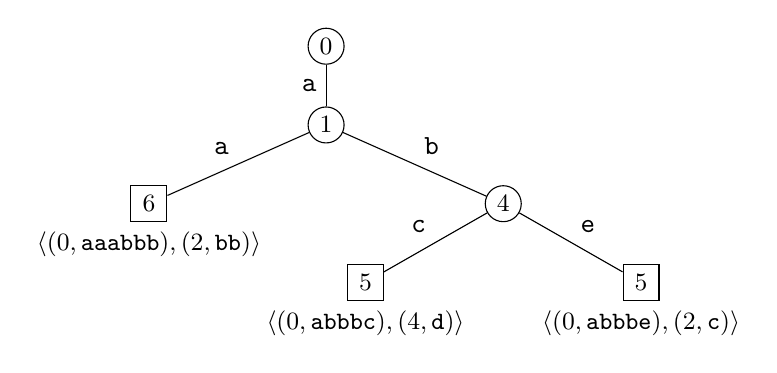
\begin{tikzpicture}[
      grow=down,
      inner/.style={draw, fill=white, inner sep=0, minimum size=13, circle},
      leaf/.style={draw, fill=white, inner sep=0, minimum size=13},
      level 1/.style={level distance = 1cm},
      level 2/.style={sibling distance = 4.5cm, level distance = 1cm},
      level 3/.style={sibling distance = 3.5cm, level distance = 1cm}
    ]
    \node[inner] {\small 0}
      child {
        node[inner] {\small 1}
        child {
            node[leaf, label=below:{\small $\langle (0, \text{\tt aaabbb}), (2, \text{\tt bb}) \rangle$}] {\small 6}
            edge from parent[-] node[above left] {\tt a}
        }
        child {
            node[inner] {\small 4}
            child {
                node[leaf, label=below:{\small $\langle (0, \text{\tt abbbc}), (4, \text{\tt d}) \rangle$}] {\small 5}
                edge from parent[-] node[above left] {\tt c}
            }
            child {
                node[leaf, label=below:{\small $\langle (0, \text{\tt abbbe}), (2, \text{\tt c}) \rangle$}] {\small 5}
                edge from parent[-] node[above right] {\tt e}
            }
            edge from parent[-] node[above right] {\tt b}
        }
        edge from parent[-] node[left] {\tt a}
      };
    \end{tikzpicture}

    \caption{Graphical representation of the 2-level index built over $S_0$,
    $S_2$ and $S_4$, with the underlying Front-Coding.}

    \label{fig:2-level-index}
  \end{figure}

  \item We first perform a \emph{blind-search} on the Patricia trie for the
  string $P = \text{\tt aaabba}$, obtaining a partial match on its first and
  second character ({\tt \underline{aa}abba}). The string pointed by the
  Patricia trie is $S_0 = \text{\tt aaabbb}$, which is the first string in the
  block but also of the entire trie. It has a common prefix with $P$ of length
  $\ell = 5$, and since $P[\ell + 1] < S_0[\ell + 1]$, we do not have to
  uncompress the front-coding and we can state that $\forall s \in S.\ P \prec
  s$.

\end{enumerate}
